
\begin{figure}
\centering
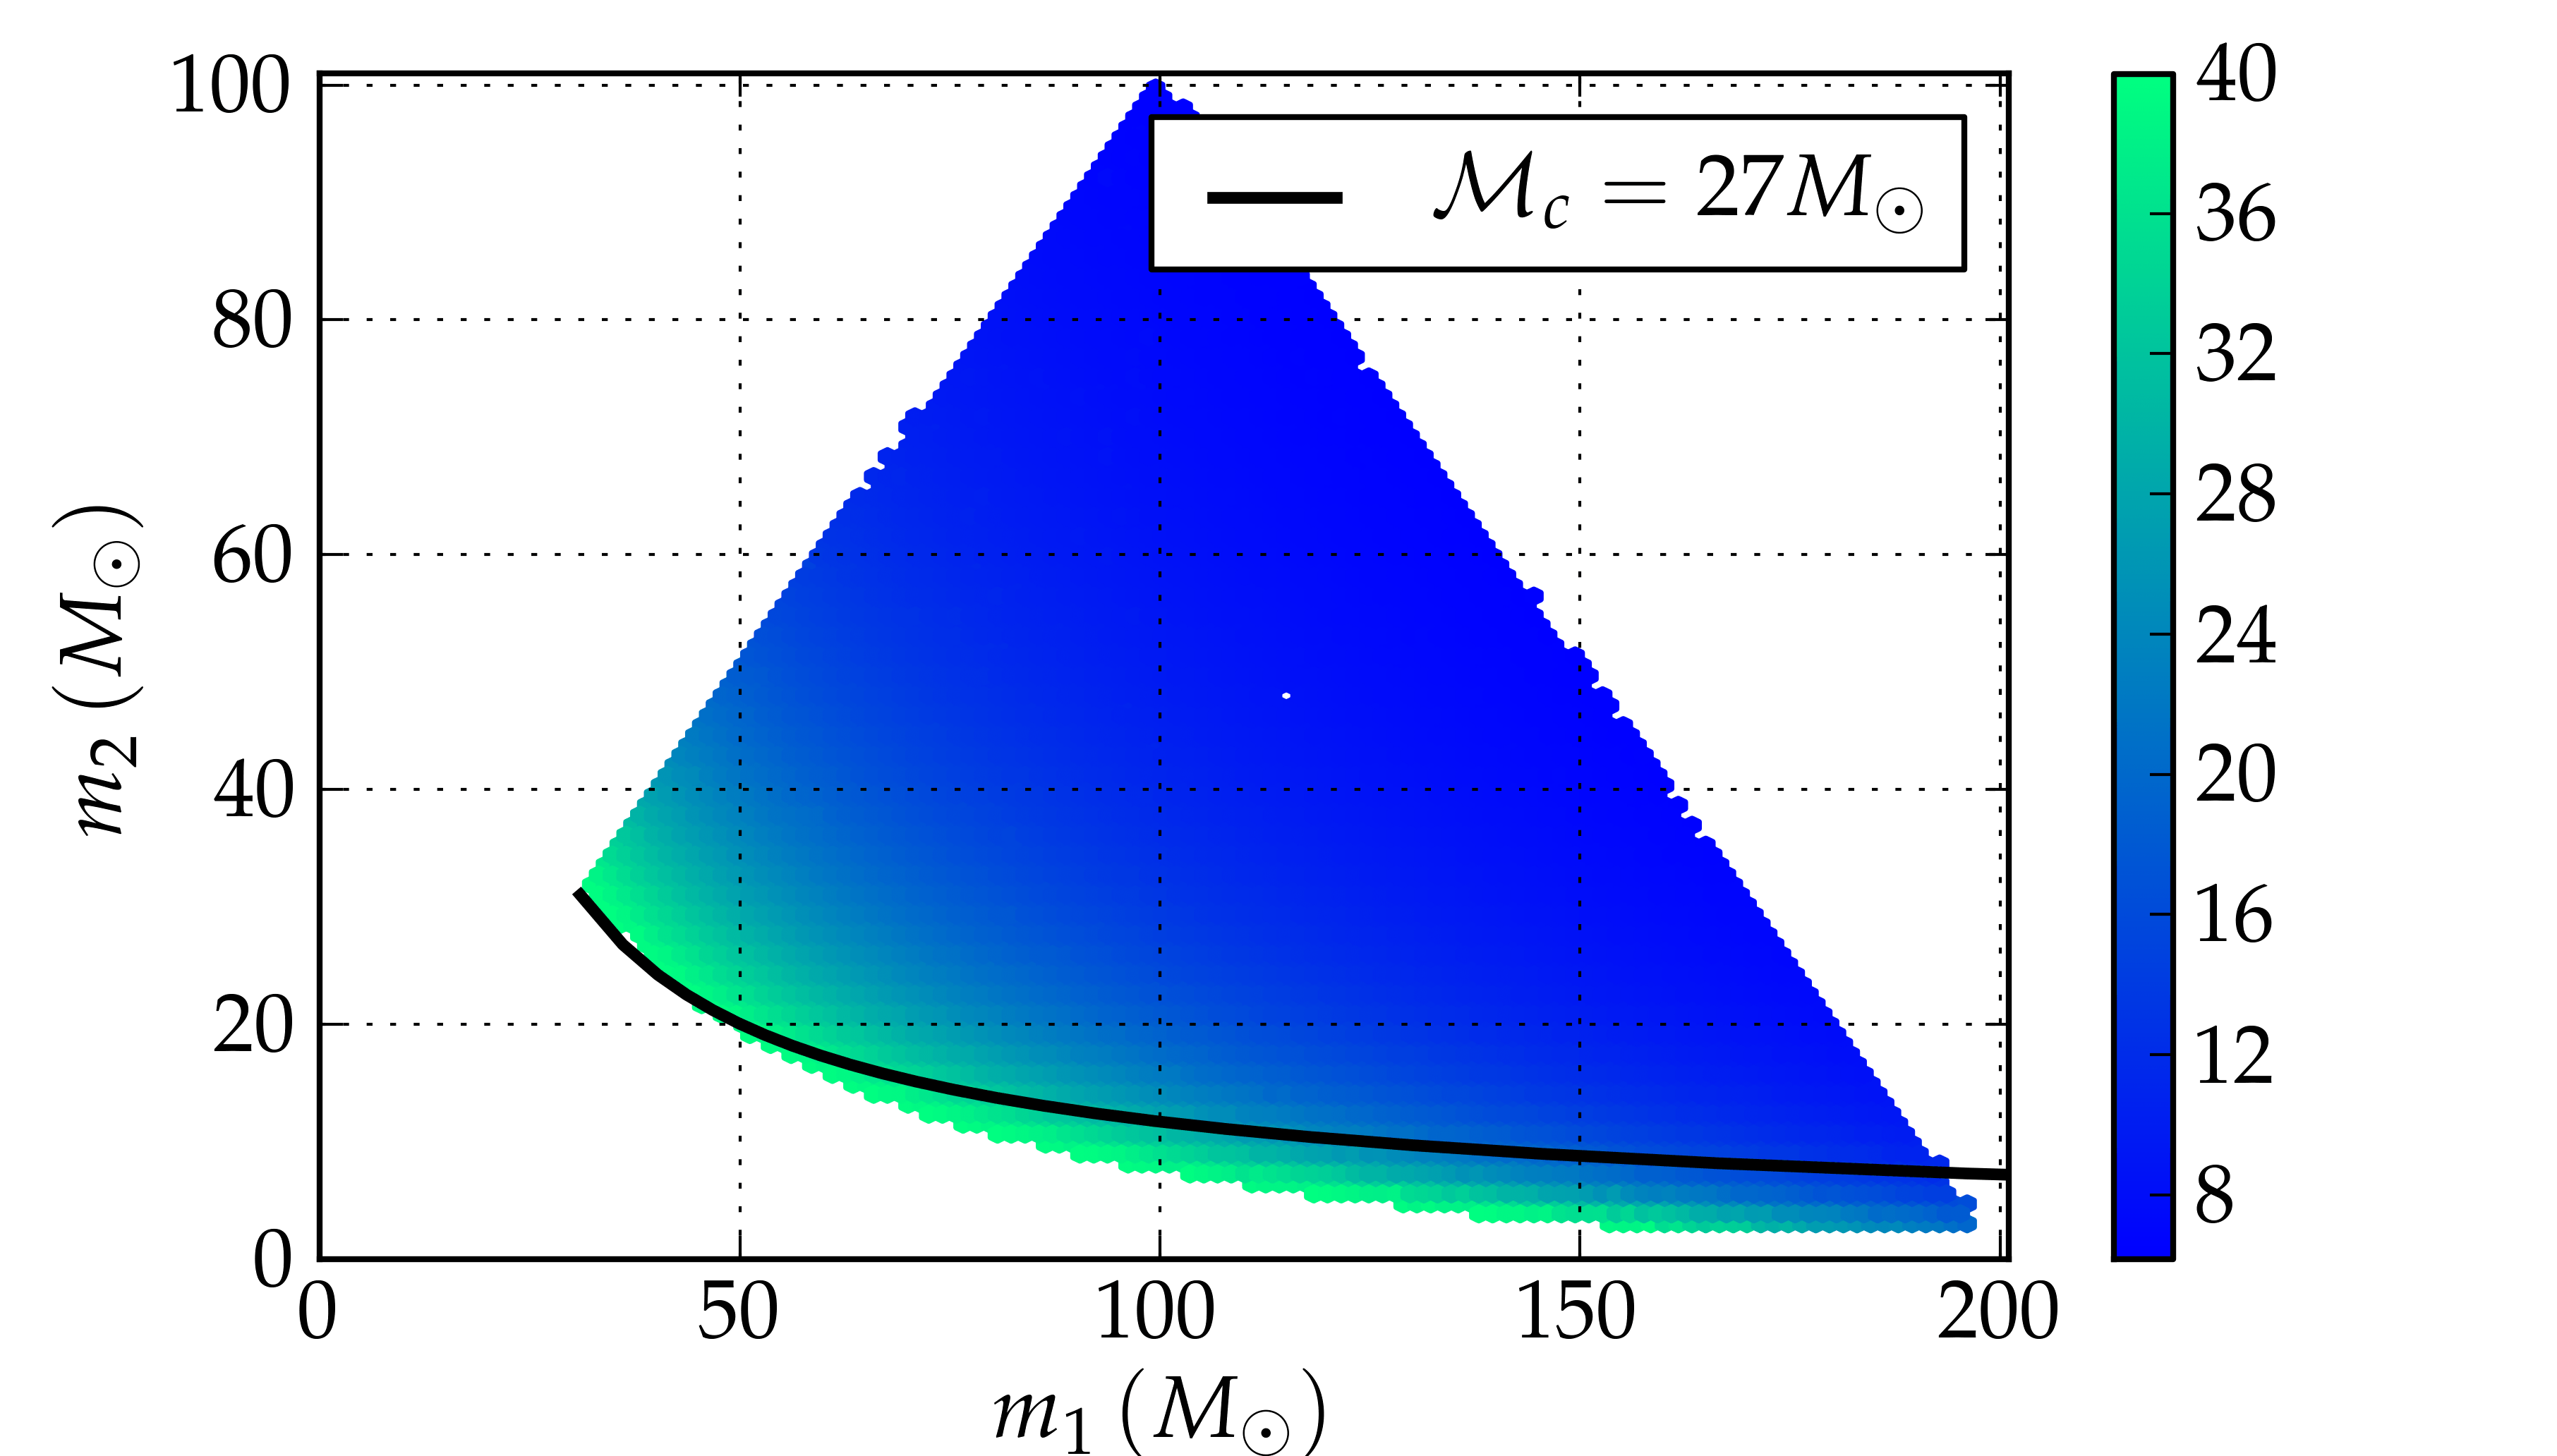
\includegraphics[width=1.1\columnwidth]{BBHm1m2_tlen_Ncyc40_0-99_Mchirp27_cropped-tiny.png}%\quad
%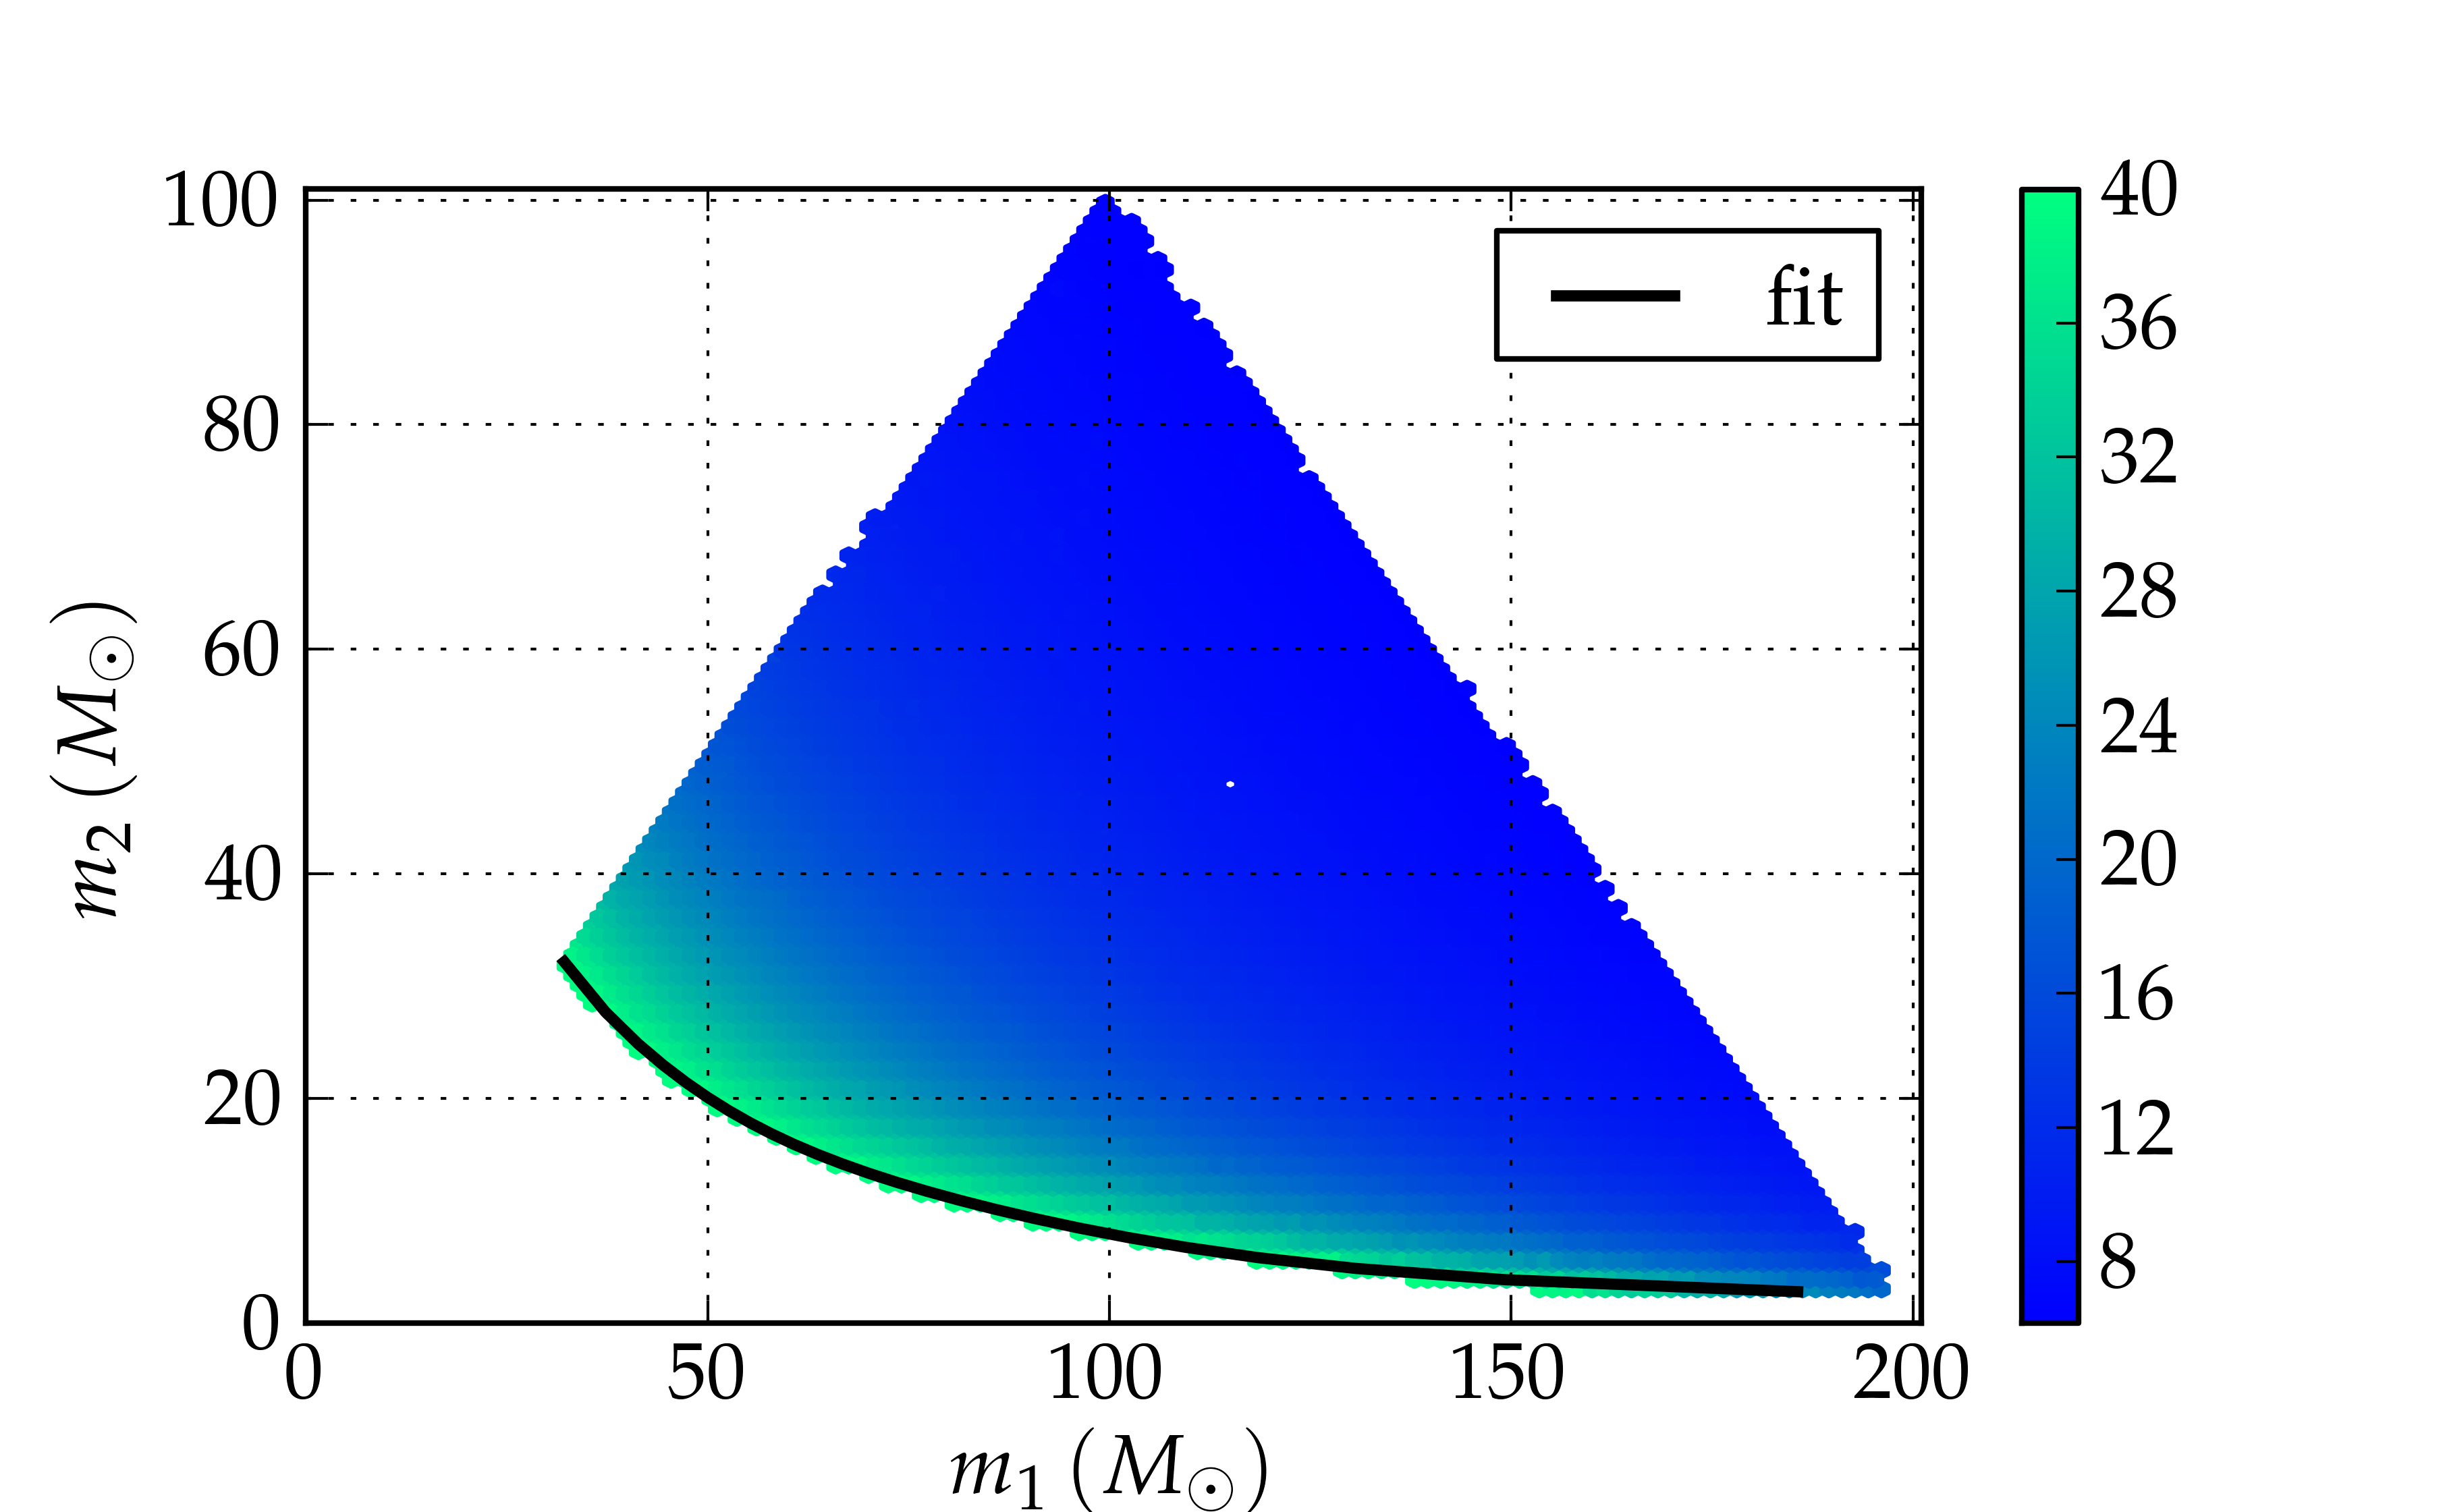
\includegraphics[width=\columnwidth]{BBHm1m2_0-99power_Ncyc40.png}
\caption{The color at each point gives the number 
of waveform cycles $\N_{\cyc}$, for that particular binary, which contain 
$99\%$ of the signal power in the aLIGO sensitivity band. The figure is 
trucated to exclude the region where $\N_{\cyc}>40$. The solid curve shows
the lower bounding edge of the region with $\mathcal{M}_c = 27M_\odot$.}
\label{fig:BBHregion}
\end{figure}

In this section we demonstrate the effectualness of a template bank viable
for using NR waveforms as templates. The gravitational-wave phase of the dominant 
waveform multipole 
extracted from runs at different resolutions was found to converge within 
$\sim 0.3\,\mathrm{rad}$ for $q=3,4,6$, and within $\sim 0.06\,\mathrm{rad}$
for $q=1,2$ at merger (see Fig.~(6) of Ref.~\cite{Buchman:2012dw}, and 
Fig.~(6,7) of Ref.~\cite{BuonannoEOBv2Main} for a compilation). Most of this 
phase disagreement accumulates over a relatively short duration of 
$\sim 50M  - 100M$ before merger, and is significantly lower over the preceding
inspiral and plunge. As the matched-filter SNR accumulates secularly over the
entire waveform, 
these numerical phase errors are negligible in terms of mismatches. We set
$\Gamma_\Hyb = 0$ while computing the fitting factors, so one is left with
considering $\Gamma_\bnk$ to determine the fidelity of the bank (c.f.
Eq.~(\ref{eq:FFGammas})).
% \red{[Harald: These figures compare EOB with NR.  
% How does this imply a statement about the accuracy of the NR waveforms?]}.
% \textcolor{blue}{This was left out at this place by error. The original
% context was the justification of using EOBNRv2 waveforms as
% proxies for NR simulations. I have removed it here.}

With NR simulations as templates, the region that the bank can cover is 
restricted to binaries that have approximately the same number of waveform 
cycles within the sensitive frequency band of the detectors as the simulations
themselves. We take their fiducial length to be $\sim 40$ GW
cycles~\cite{40GWcycles}. For BBHs with 
$3M_{\odot}\leq m_1,m_2\leq 200M_{\odot}$ and $m_1+m_2\leq 200M_{\odot}$ 
we map out the region with $99\%$ of the signal power within $40$ cycles as the
target region of the purely-NR bank. For samples taken over the mass space, we
determine the frequency interval $[f_1,f_2]$ for which
\begin{equation}\label{eq:99percentpower}
 \int_{f_1}^{f_2}\D f \dfrac{|\tilde{h}(f)|^2}{S_n(|f|)} = 
0.99\times\int_{f_\mathrm{min}}^{f_\mathrm{Ny}}\D f \dfrac{|\tilde{h}(f)|^2}{S_n(|f|)}.
\end{equation}
This is done by finding the peak of the integrand in 
Eq.~(\ref{eq:99percentpower}) and integrating symmetrically outwards from 
there, in time, till the interval $[f_1,f_2]$ is found. The number 
of waveform cycles in this interval is
\begin{equation}
 \N_{\cyc} = \dfrac{\Phi( t(f_2) ) - \Phi( t(f_1) )}{2\pi},
\end{equation}
where $\Phi(t)$ is the instantaneous phase of the waveform, 
${h_+(t)\,-\,\ii h_{\times}(t)\,=\,A(t)\,e^{-\ii \Phi(t)}}$, un-wrapped to be a
monotonic function of time. 
We find that for a significant portion of the mass-region, the signal power 
is contained within $40$ waveform cycles. This is shown in 
Fig.~\ref{fig:BBHregion}, where the color at each point gives $\N_{\cyc}$ for
that system, and the region with $\N_{\cyc}> 40$ is excluded. Conservatively, 
this region is bounded by $\mathcal{M}_c = 27M_\odot$, as shown by the solid 
curve in the figure.
% A fit for the total mass $M$ at the lower boundary of this region is given by
% \begin{equation}\label{eq:MtotalFit40Cycles}
% \begin{split}
%  M = \eta^{-3/5}&(12.02 + 217.76\eta - 1469.6\eta^2 + 5169.4\eta^3\\  
%  &-7011.5\eta^4),
%  \end{split}
% \end{equation}
% where $\eta = m_1m_2/M^2 = q/(1+q)^2$ is the symmetric mass-ratio.
% \red{[Harald: Eq (37) is very complicated.  It would be good to
%   give a simpler ``rule-of-thumb''.  By playing around, I found that
%   for the mass-ratios we are interested in, ${\cal M}_c=\mbox{const}$
%   works reasonably well.  I suggest to find the constant, point out that ${\cal M}_c\gtrsim XX$ is an approximation for $q<YY$, and also plot it in Fig. 3.]}


We place a bank over this region, using a stochastic method similar 
to Ref.~\citep{Harry:2009ea,Ajith:2012mn,Manca:2009xw}. 
The algorithm begins by taking an empty bank,
corresponding to step $0$. At step $i$, a proposal point $(q,M)$ is picked
by first choosing a value for $q$ from the restricted set
$\mathcal{S}_q=\{1,2,3,4,6,8\}$. The total mass $M$ is subsequently sampled
from the restricted interval corresponding to the pre-drawn $q$. The proposal 
is accepted if the waveform at this point has overlaps $\mathcal{O}< 0.97$ 
with all the templates in the bank from step $i-1$. This gives 
the bank at step $i$. The process is repeated till the fraction of 
proposals being accepted falls below $\sim 10^{-4}$, and $\gtrsim 99\%$
of the parameter space is covered effectually.
% \red{[Harald: I would have expected that by the time such a small acceptance fraction is reached, the bank is complete.  Is there a simple explanation why not?]}
% \textcolor{blue}{The acceptance rate decreases extremely rapidly as the bank
% converges to $> 99\%$ coverage fraction. This was shown in
% http://arxiv.org/abs/0908.2090 (Table II and Fig. 9). Table II
% shows that an acceptance ratio of $1$ in $10^4$ is achieved close to a 
% coverage fraction of $99.9\%$, while sampling in $\tau_0 - \tau_3$ coordinates.
% We can expect it to be lower for us as we sampled in $\mathcal{M}_c - \eta$ 
% coordinates.}
To complete the coverage, $100,000$ points are sampled over the region of mass
space depicted in Fig.~\ref{fig:BBHregion}, and $\FF$ of the bank
is computed at each point. With the islands of undercoverage isolated, the
points sampled in these regions are added to the bank, pushing their 
mass-ratios to the two neighboring mass-ratios in $\mathcal{S}_q$ 
along lines of constant chirp mass. 
This helps accelerate the convergence of the bank, albeit at the cost of 
over-populating it, as the algorithm for computing the $\FF$ for the 
sampled points is parallelizable.
\begin{figure}
\centering
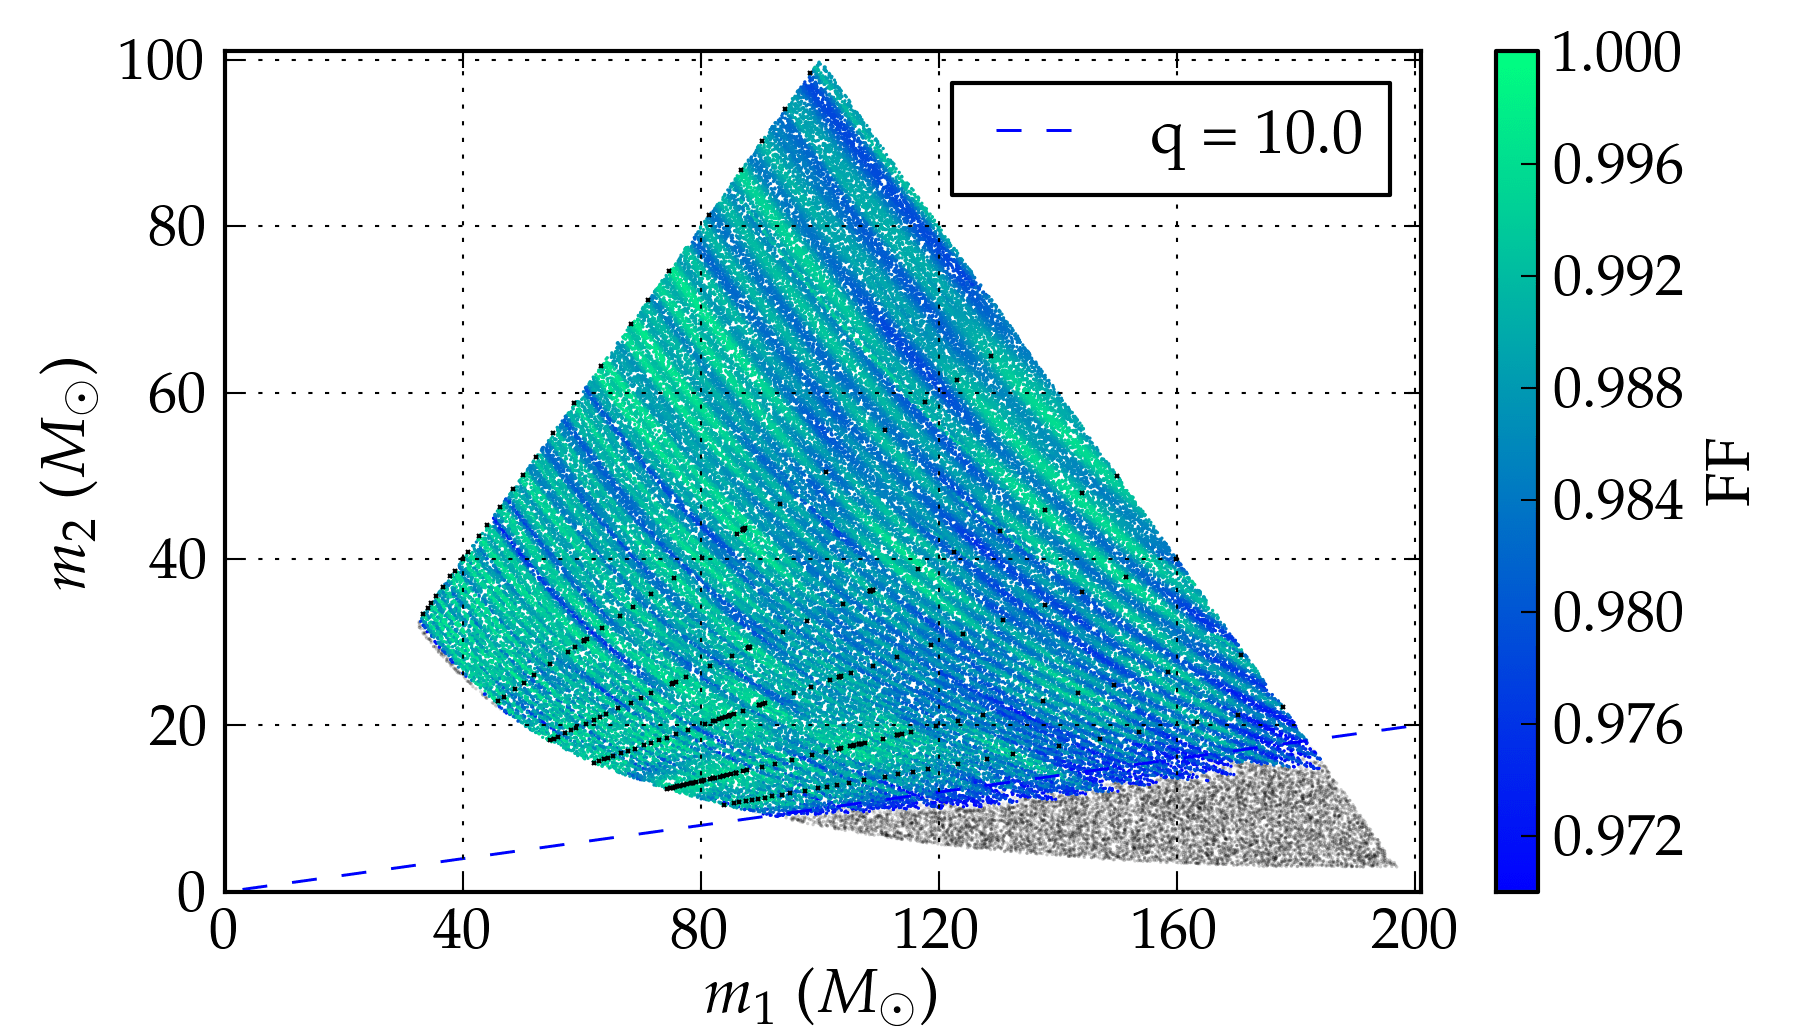
\includegraphics[width=\columnwidth]{bank002_01_01_mtot200_match_cropped-tiny.png}
%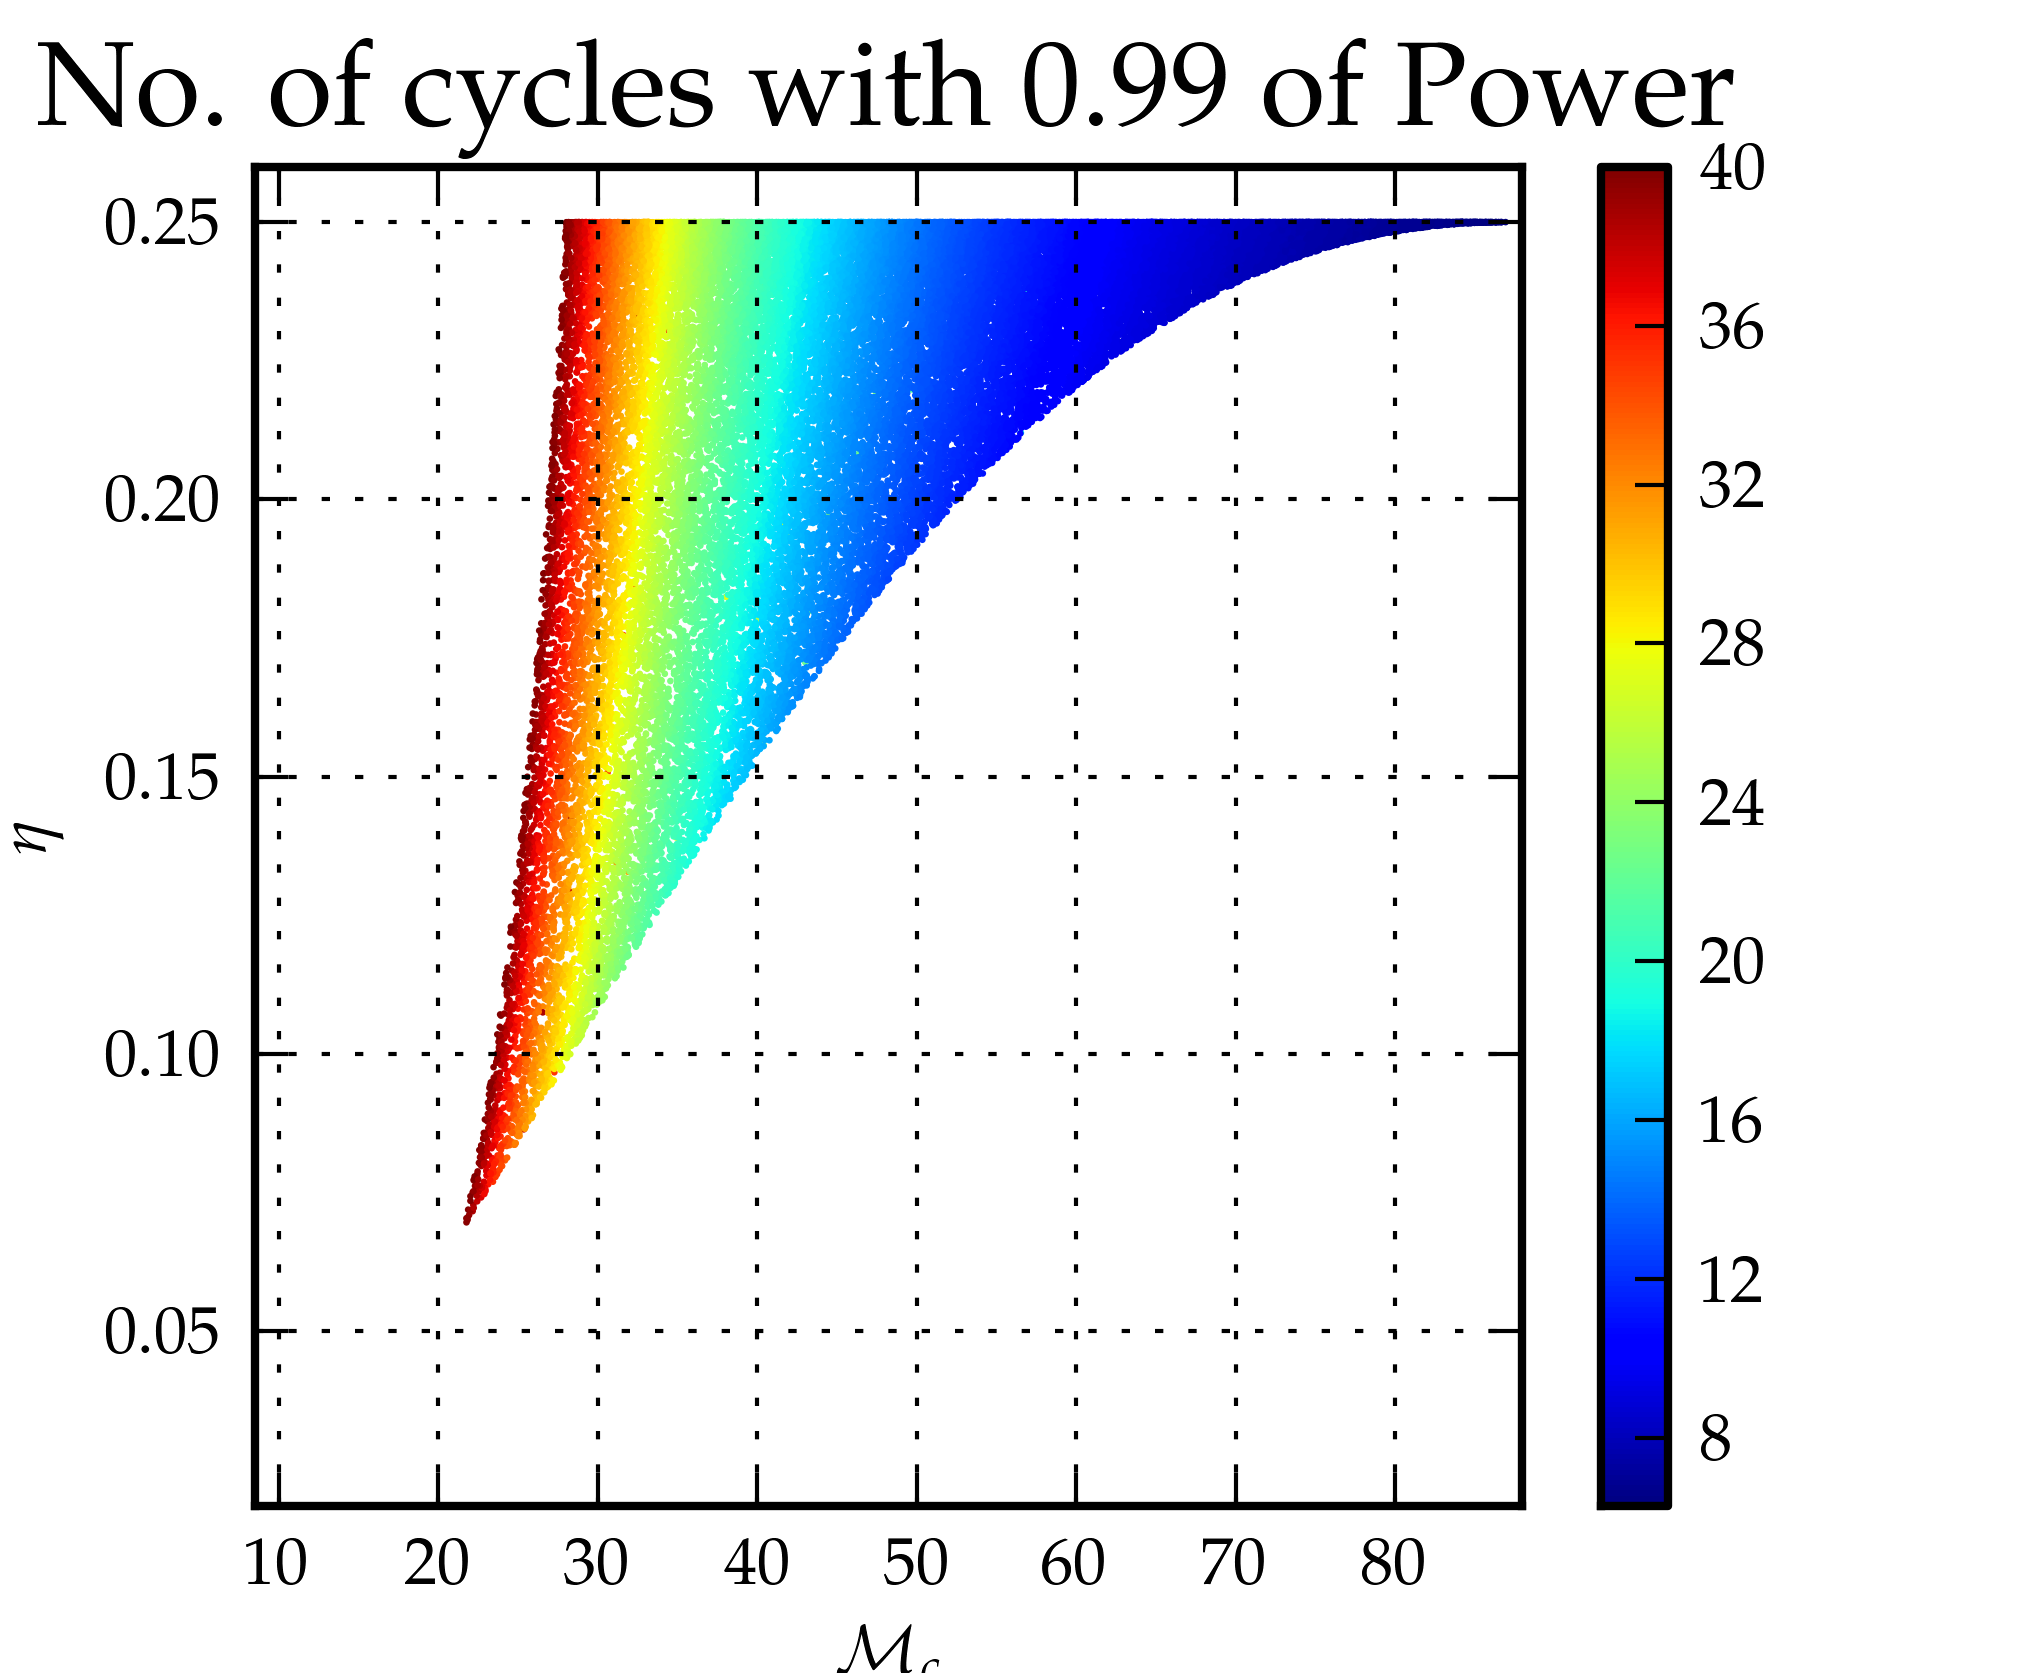
\includegraphics[width=\columnwidth]{BBHmcet_0-99power_Ncyc40.png}
\caption{The color at each point in the figure gives the
value of $\FF\simeq 1-\Gamma_{\bnk}$ of the bank for that binary, for
the NR bank restricted to $\mathcal{S}_q=\{1,2,3,4,6,8\}$. This is the
same as the fraction of the optimal SNR, for the binary, that the
template bank recovers. The black dots show
the location of the templates in the bank. We note that they all lie
along straight lines of constant $q$ passing through the origin. The region 
shaded light-grey (towards the bottom of the figure) is where the $\FF$ 
drops sharply below $97\%$.}
\label{fig:bank001_01_match}
\end{figure}
\begin{figure}
\centering
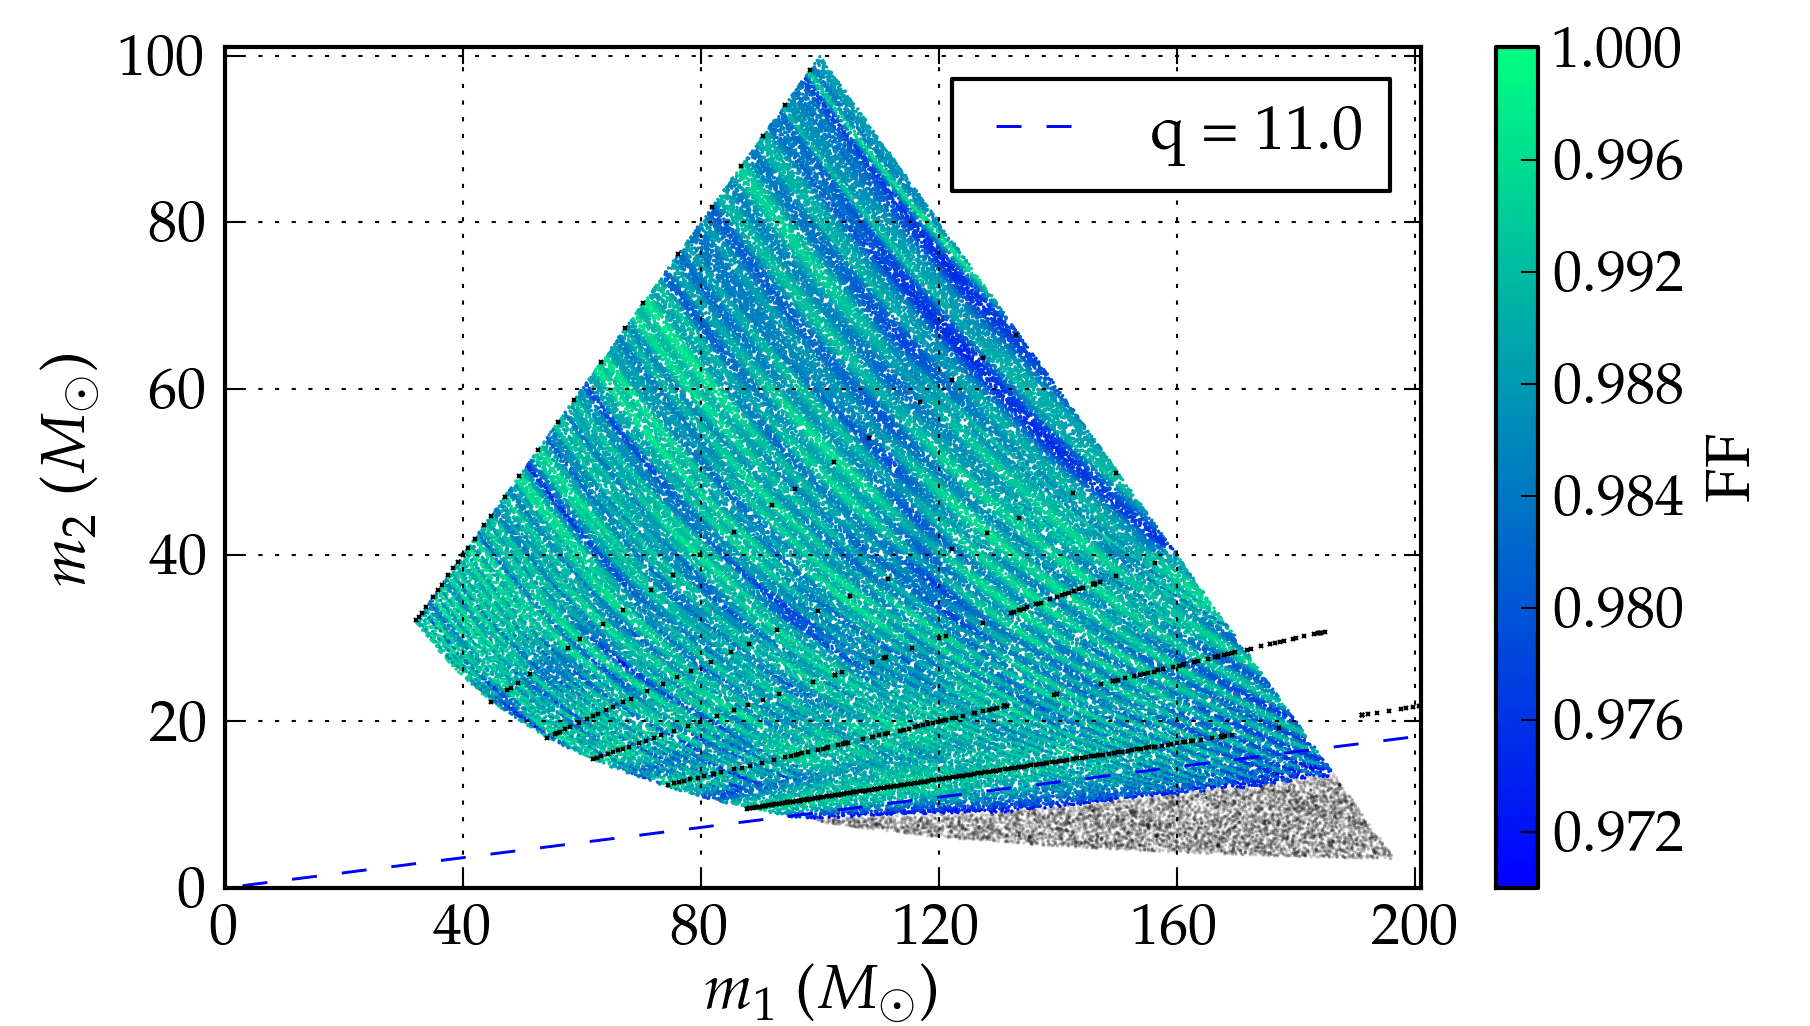
\includegraphics[width=\columnwidth]{bank006_01_mtot200_match_cropped-tiny.png}
%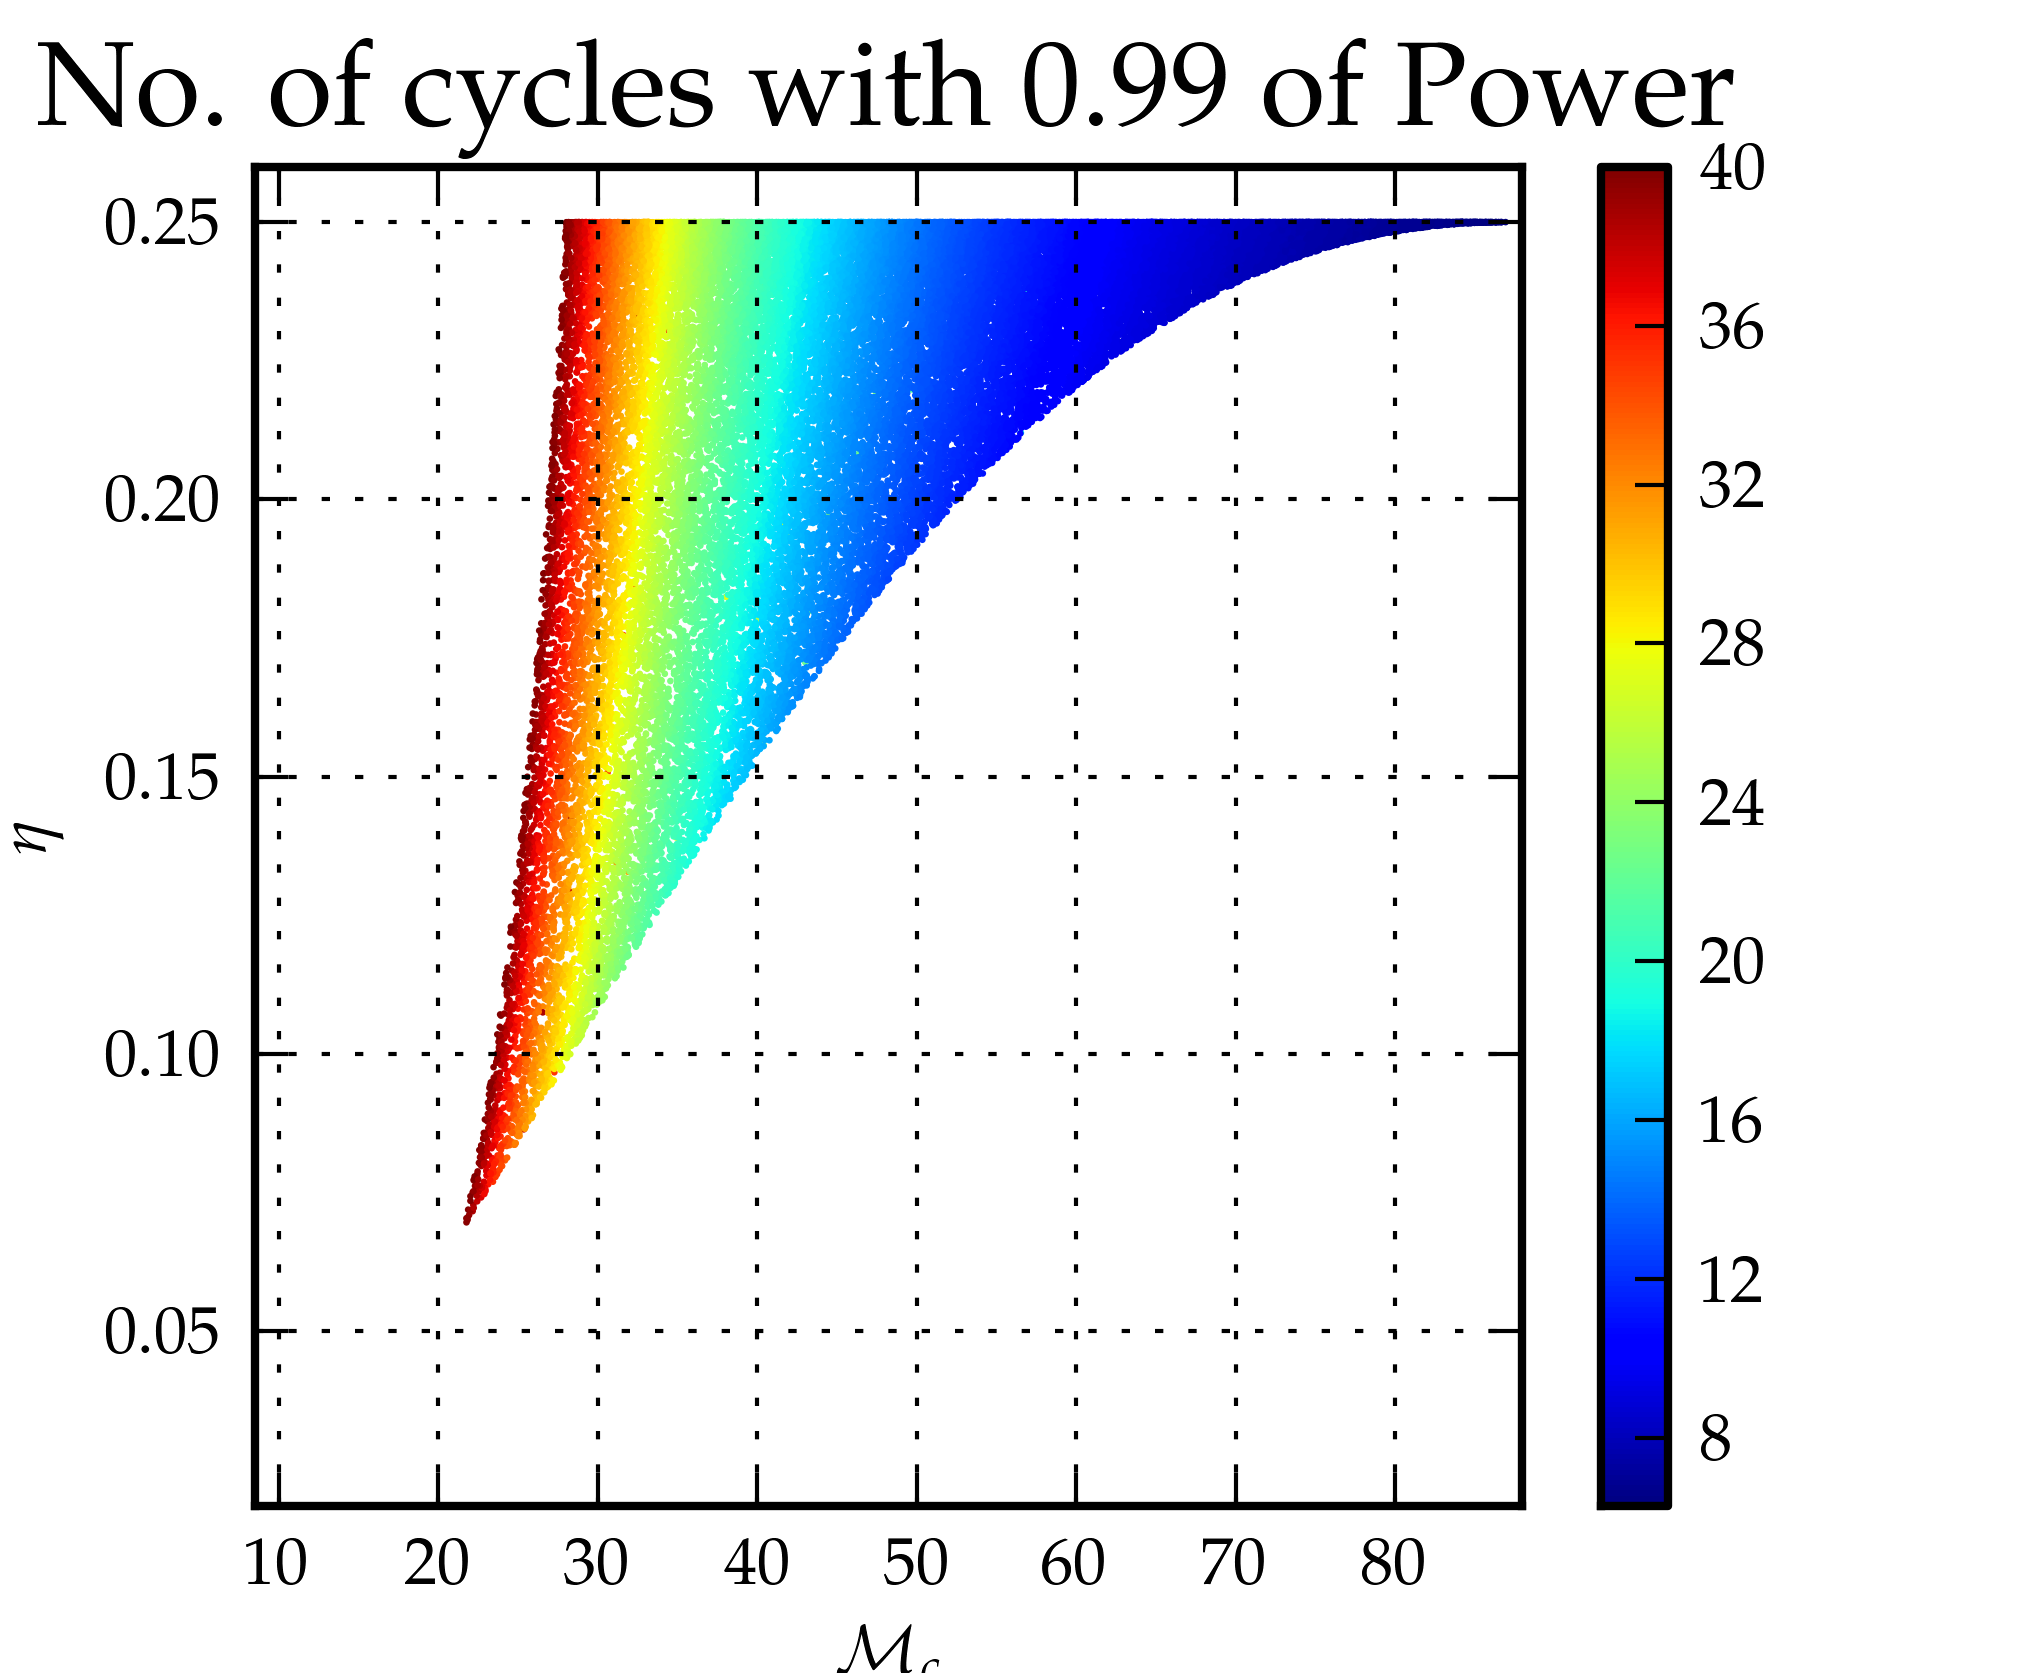
\includegraphics[width=\columnwidth]{BBHmcet_0-99power_Ncyc40.png}
\caption{This figure is similar to Fig.~\ref{fig:bank001_01_match}.
The color at each point gives the value of 
$\FF\simeq 1-\Gamma_{\bnk}$ of the bank for that binary, for
the NR bank restricted to $\mathcal{S}_q=\{1,2,3,4,6,9.2\}$.
The black dots show the location of the templates in the bank. 
The region shaded light-grey (towards the bottom of the figure) is 
where the $\FF$ drops below $97\%$. We note that with an additional
NR waveform for mass ratio $q=9.2$, the coverage of the bank is 
extended to include binaries with $10\leq q\leq 11$.}
\label{fig:bank006_01_match}
\end{figure}
% We test the bank so constructed by measuring the loss in the SNR that the 
% bank incurs for arbitrary incoming GW signals. As the waveform 
% mismatches due to the numerical errors are negligibly small, the primary cause
% for the loss in SNR would be the discreteness of the template bank grid. This
% effect can be measured by simulating BBH waveforms for various systems sampled
% over the region of the mass-parameter space that the bank intends to cover, and
% computing the fraction of optimal SNR that is recovered when these signals are
% filtered with our bank. 
% We need the signals and templates to be in the same
% manifold, to measure the effect of the discreteness of the bank alone.
% The recently proposed EOBNRv2 approximant~\cite{BuonannoEOBv2Main} was 
% calibrated to the numerical simulations for $q=\{1,2,3,4,6\}$, and thus 
% provides an excellent ground for that, i.e. superscript M~=~EOBNRv2 in
% $\Gamma_{\bnk}$ (Eq.~\ref{eq:FFConstraint}).

We asses the effectualness of the bank, as discussed in 
Sec.~\ref{s1:quantifyingerrors}, using Eq.~(\ref{eq:NRFFGammas}).
We draw a population of $100,000$ BBH signals, uniformly from the binary 
mass space, and filter them through the bank. Fig.~\ref{fig:bank001_01_match}
shows the $\FF$, or the fraction of the optimal SNR recovered by the bank. 
The region shown is restricted to binaries with $N_{\cyc}\leq 40$.
The black dots in the figure show the position of templates in the bank. 
The bank recovers $\geq 97\%$ of the optimal SNR over the entire region 
of interest for $q\leq 10$. We 
propose an additional simulation for $q=9.2$, to increase the coverage to
higher mass-ratios. Substituting this for $q=8$ in the set of allowed 
mass-ratios $\mathcal{S}_q$, we place another bank as before, with
$\mathcal{S}_q=\{1,2,3,4,6,9.2\}$. The SNR loss from this bank is shown in
Fig.~\ref{fig:bank006_01_match}. This bank recovers $\geq 97\%$ of the SNR for
systems with $q\leq 11$ and $\N_{\cyc}\leq 40$. The choice of the additional
simulation at $q=9.2$ was made by choosing a value \textit{close-to} the 
highest possible value of $q$ that does not lead to under-coverage in the 
region between $q=6$ and that value. The \textit{exact} highest allowed 
value was not chosen to reduce the sensitivity of the coverage of the bank
to fluctuations in detector sensitivity.

We conclude that with only six NR waveforms for non-spinning BBHs, that are
$\sim 20$ orbits (or $40$ GW cycles) in length, a template bank can be
constructed that is effectual for detecting binaries with chirp mass above
$27M_\odot$ and $1\leq q\leq 10$. With an additional 
simulation for $q=9.2$, this bank can 
be extended to higher mass-ratios, i.e. to $1\leq q\leq 11$.

